% This is samplepaper.tex, a sample chapter demonstrating the
% LLNCS macro package for Springer Computer Science proceedings;
% Version 2.20 of 2017/10/04
%
\documentclass[runningheads]{llncs}
%
\usepackage{graphicx}
% Used for displaying a sample figure. If possible, figure files should
% be included in EPS format.
%
% If you use the hyperref package, please uncomment the following line
% to display URLs in blue roman font according to Springer's eBook style:
% \renewcommand\UrlFont{\color{blue}\rmfamily}

\usepackage{times}
\usepackage{graphicx}
\usepackage{latexsym}
\usepackage{amsmath}
\usepackage{algorithm}
\usepackage{algorithmicx}
\usepackage{amsfonts}
\usepackage{amssymb}
\usepackage{bm}
\usepackage{multirow}
\usepackage{threeparttable}

\begin{document}
%
\title{Synthesis of Registered Multimodal
		Medical Images with Lesions}
%
%\titlerunning{Abbreviated paper title}
% If the paper title is too long for the running head, you can set
% an abbreviated paper title here
%\inst{1}
\author{ Yili Qu \and Wanqi Su \and Chufu Deng \and Ying Wang \\
	\and Yutong Lu \and Zhiguang Chen \and Nong Xiao}
%
\authorrunning{Yili, Wanqi et al.}
% First names are abbreviated in the running head.
% If there are more than two authors, 'et al.' is used.
%
\institute{Sun Yat-sen University,	China,\\
	\email{quyli,suwq7,chufd3@mail2.sysu.edu.cn}}
%
\maketitle              % typeset the header of the contribution
%
\begin{abstract}
In a large number of data-driven medical image intelligent processing tasks, the collection and annotation of medical image data is very difficult, especially registered multimodal medical image data. Synthetic medical image data can alleviate the problem of insufficient data well. In this paper, based on the unsupervised conditional GAN model, we achieve the synthesis of registered multimodal medical images from a random normal distribution matrix, and the corresponding lesion information can be efficiently generated based on the freely selected lesion label. We conduct a number of validation experiments on multiple datasets to verify that our synthetic images can be used as pre-trained data or enhanced data in medical image intelligent processing tasks, and they can greatly improve the generalization ability of the model.

\keywords{Image Synthesis \and  Multimodal \and Medical Images \and  Lesions.}
\end{abstract}
%
%
%
\section{Introduction}
In recent years, intelligent medical image processing has become one of the most influential fields in the application of deep learning. Medical images is the images of biological tissue used in medical treatment. Medical images obtained using different imaging methods are called different modalities. The common modalities include magnetic resonance imaging (MRI), CT, X-ray, etc. Some modalities are divided into different submodalities according to different settings during imaging, such as MRI including T1, T2, T1c and Flair.
More and more medical images research based on deep learning is expected to obtain a large number of medical images data. However, the collection and annotation of medical image data is very difficult, especially for the registration of multi-mode data. With the development of image synthesis technology, it is possible to synthesize high-quality medical images. This is a good way to alleviate the scarcity of medical images data.
However, medical images contain complex physiological structure information, and the usual way of synthesis is likely to produce unreasonable structure or contour. On the other hand, the researchers expect multimodal medical images to provide more information for diagnosis. It is also a challenge to ensure the registration of composite image when multimodal image is synthesized.
Most importantly, the greatest value of medical images is the lesions information. The lesions information in medical images is an important basis for doctors to make diagnosis, s well as an important basis for reasoning and diagnosis of intelligent medical image processing model. Therefore, another big challenge in synthesizing medical images is to control the synthesis of lesions and generate corresponding lesion labels.


%Before the proposal of deep learning, some studies used methods such as map dictionary mapping\cite{22burgos2015robust} and sparse coding\cite{33huang2017simultaneous,34vemulapalli2015unsupervised} to carry out the initial attempts of medical image synthesis. After deep learning was proposed, some studies were based on CNN's synthetic medical images \cite{66miao2018dilated,36vannguyen2015crossdomain}.
With the development of gan-based image synthesis, GAN has gradually been widely used in medical image segmentation\cite{40kamnitsas2017unsupervised}, reconstruction\cite{61fan2018a,65anirudh2018lose}, synthesis \cite{4shin2018medical,41costa2017towards,43iglesias2013is,44shrivastava2017learning}, translation \cite{2zhang2018translating,20nie2017medical,35osokin2017gans,36vannguyen2015crossdomain,40kamnitsas2017unsupervised,136yi2018sharpness-aware,137yang2018low-dose,138WolterinkGenerative} and super resolution \cite{14You2018CT,15lyu2018super-resolution}. 
%Some studies on medical image synthesis through mode conversion aim to reduce the radiation dose of patients by synthesizing high-dose CT with non-radiation MRI or low-dose CT with low radiation\cite{2zhang2018translating,20nie2017medical,136yi2018sharpness-aware,137yang2018low-dose,138WolterinkGenerative}.

Recently, some studies have attempted to alleviate the difficulty of having few samples of medical image data by synthesizing more diverse data, such as the synthesis of brain MRI\cite{4shin2018medical}, the synthesis of retina \cite{41costa2017towards}, and the synthesis of monomorphic medical images of many different parts and modes\cite{96zhang2019skrgan:}. Among them, the brain MRI synthesis \cite{4shin2018medical} GAN synthetic brain images is applied to implement the image through synthetic data enhancements and anonymous, but its input is extracted from real data structure division of the brain, not only need additional training in tabbed and split, you also need to provide segmentation result in another data set, which makes this method is restricted by many factors. In this study, tumor segmentation tags were added at the time of input for the first time to guide the synthesis of lesions. However, there were no additional constraints during the synthesis process, making the synthesis of lesions extremely uncertain. Retinal synthesis studies\cite{41costa2017towards} achieved the random generation of vascular annotation images by variational self-encoder (VAE) \cite{87kingma2014auto-encoding,88rezende2014stochastic}, and then the color retinal images were synthesized with the synthesized vascular annotation images. The latest SkrGAN\cite{96zhang2019skrgan:} made a monomodal image synthesis attempt, and in line with this research idea, Sobel operator was used to extract sketches containing structural information from medical images, and then further synthesizes medical images. However, similar to other studies, the medical images synthesized by SkrGAN did not consider the synthesis of lesion information or the production of corresponding lesion labels, which made most of the synthesized data unavailable.

To solve these problems, we design a multimodal medical image synthesis scheme based on ACGAN\cite{98odena2016conditional}.  Our solution can receive a random normal distribution matrix as input to synthesize a set of registered multimodal MRI images with specify lesions. We conducted synthesis experiments on several public datasets, which fully verified the effectiveness of synthetic lesions and the availability of synthetic data. Our main work includes the following aspects:
\begin{itemize}
	\item Compared with the current best sketch extraction method, we proposed a more concise and clear structural map extraction method based on Sobel Operator\cite{147Sobel}, which can directly extract anatomical structure information from medical images without training or other label data.
	
	\item We propose a method based on VAE and GAN, which can synthesize any number of more diverse structural feature graphs from multi-dimensional normal distribution random sampling, and can synthesize the structural feature graphs satisfying the expected structure style by controlling the sampling sites in the normal distribution.
	
	\item We propose a new method for synthesizing multimodal medical images with lesions by adding lesion tags. The loss constraint generation model provided by the lesion processor corresponds to the lesion according to the tag synthesis, and the loss constraint multimodal images provided by the modality translation network  can be registered with each other without the need of registration training data.
	
	\item We use synthetic data to train the intelligent medical image processing model, verify the effectiveness of synthetic lesions and the availability of synthetic data through the evaluation of the processing capacity of the model, and indirectly evaluate the performance and quality of synthetic images.
\end{itemize}

\section{METHOD}
\label{method}
\begin{figure}[t]
	\centering
	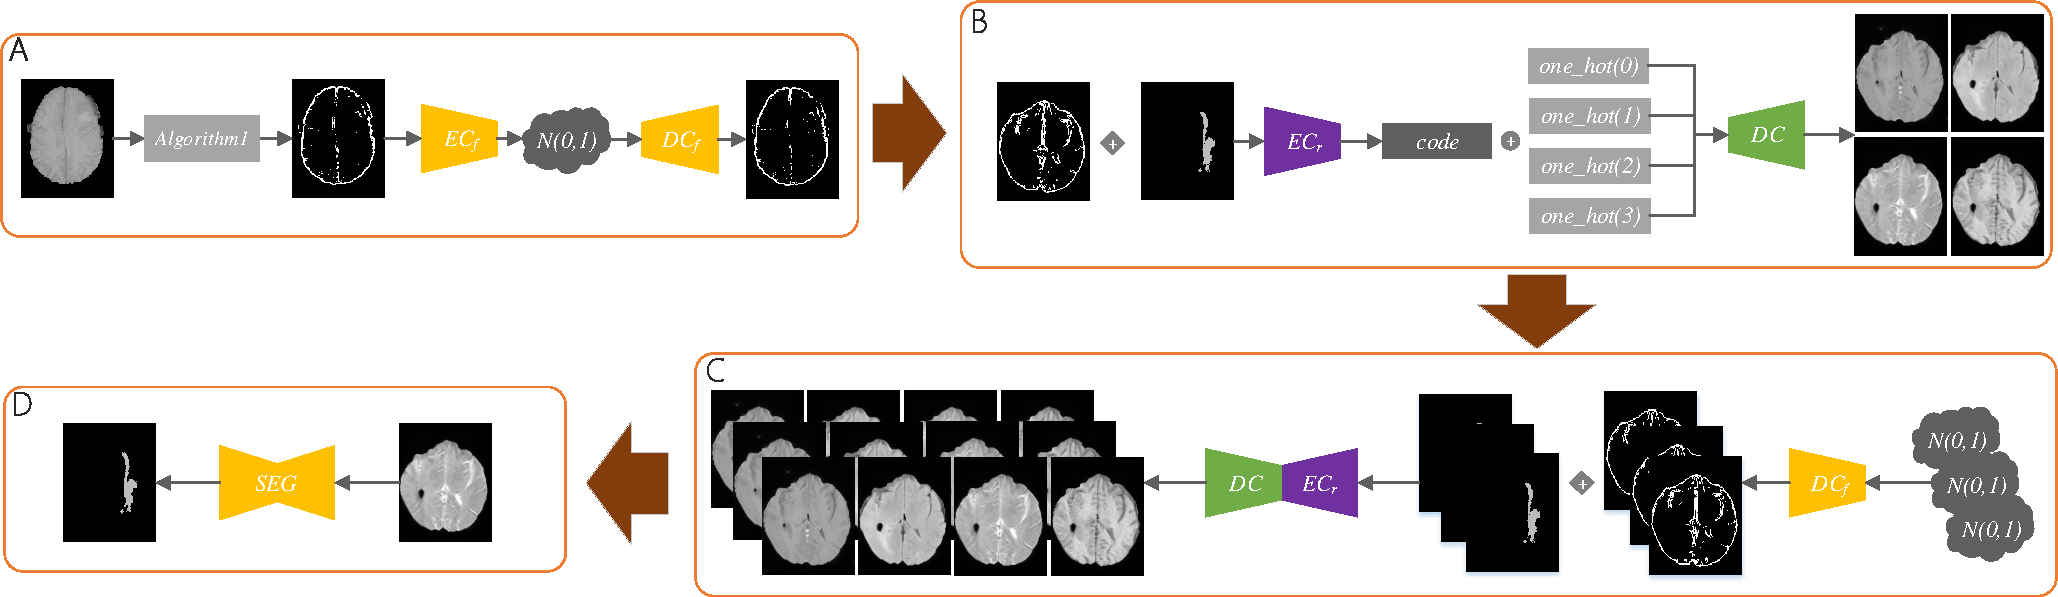
\includegraphics[width=1\textwidth]{figures/architecture}
	\caption{The overall architecture. 
%		A is the structural map extraction and generation stage. B is the multimodal MRI synthesis stage. C is the synthetic datasets construction stage. D is the synthetic data availability verification stage.
	}
	\label{architecture}
\end{figure}
As shown in Fig.~\ref{architecture}, our scheme includes four main stages. In stage A, we obtain a structural map generator that can generate structural maps from a random normal distribution matrix. 
In stage B, we train a conditional generator with input of structural maps and lesion labels, which can synthesize MRI images of different modalities according to different conditionals.
In stage C, we use the models produced in the previous stages to synthesize registered multimodal MRI images from random normal distribution matrixes. 
In stage D, we train and test the lesion segmentors on different datasets constructed from different quantities of synthetic data and real data.

\begin{algorithm}
	\caption{Structural map extraction}
	\label{alg:1}
	\begin{algorithmic}[1]
		\State Input a real grayscale image $x$,
		pixel threshold $alpha$ and $beta$ and $gama$,
		gaussian kernel variance $sigma1$ and $sigma2$
		\State $s1 = reduce\_min(sobel(x))$
		\State $s2 = reduce\_max(sobel(x))$
		\State $s1 = gaussian\_blur(s1,sigma1)$
		\State $s2 = gaussian\_blur(s2,sigma1)$
		\State $s1 = mean(s1) - s1$
		\State $s2 = s2 - mean(s2)$
		\State $s1 = ones \times (s1 > alpha)$
		\State $s2 = ones \times (s2 > alpha)$
		\State $s = ones \times ((s1 + s2)> 0)$
		\State $s = gaussian\_blur(s,sigma2)$
		\State $s = ones \times ((s1 + s2)> beta)$
		\State $s = medfilt(s)$
		\State $s = s \times (x > gama)$
	\end{algorithmic}  
\end{algorithm}
\subsection{Structural map extraction and synthesis}
We call the image that provides basic contour and structure information a structural map.  Medical images generated directly from random noise by GAN are difficult to generate realistic structural information. Structural maps can provide necessary basic guidance for the synthesis of medical images. However, general structural features such as retinal vascular maps\cite{41costa2017towards} and brain segmentation labels \cite{4shin2018medical}require additional data and training before extracting from the original image. To solve these problems, we design a method for extracting structural maps directly from brain MRI images, which has the advantages of fast operation, no training, and no additional required data. Then, we can train a generator to generate structural maps from random normal distribution matrixes.
\subsubsection{Structural map extraction method}
In traditional digital image processing methods, Roberts operator\cite{145Roberts}, Prewitt operator\cite{146prewitt}, Sobel operator\cite{147Sobel} are excellent edge detection operators. Sobel operators are particularly applicable and are most commonly used to process medical images. Algorithm~\ref{alg:1} describes our feature graph extraction method based on Sobel operator. Firstly, we use the Sobel operator to extract the horizontal and vertical edge detection maps from a real image. Each edge detection map performs maximum reduce and minimum reduce to obtain two edge detection fusion maps. Then 3$\times$3 gaussian blur was used to thicken the lines of the two images. Each fusion map calculates the difference from the average pixel value to erase  background. The two difference maps are binarized according to the pixel threshold the merge structure information. After denoising by the median filter function, the final result is the clear structural map that we need.

\begin{algorithm}
	\caption{Mask Extraction}
	\label{alg:2}
	\begin{algorithmic}[1]
		\State Input a real grayscale image $x$,  pixel threshold $alpha$, the expanded pixel value $p$
		\State $m = 1.0 - ones \times (x > alpha)$
		\State $new\_size=[x.width() + p, x.length() + p]$
		\State $m = resize(m, new\_size)$
		\State $m = crop\_padding(m,p)$
		\State $m = medfilt(m)$
	\end{algorithmic}  
\end{algorithm}
\subsubsection{Structural map generation training}
\begin{figure}
	\centering
	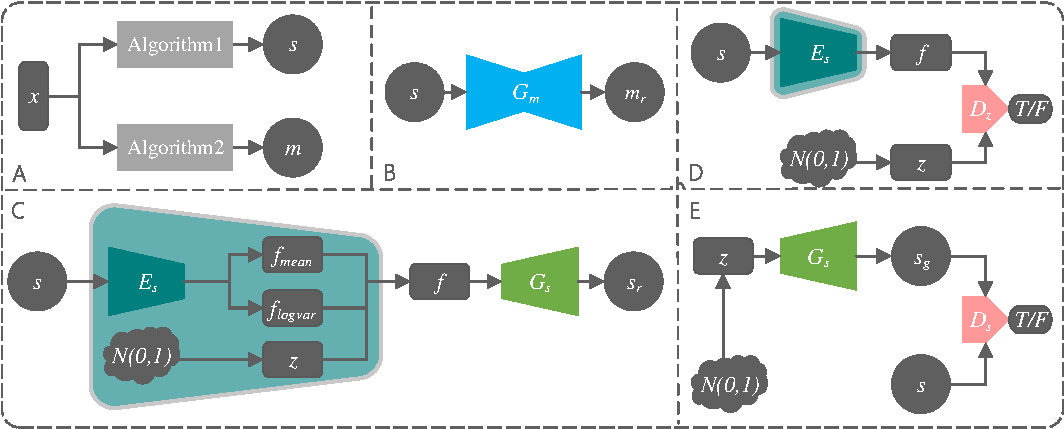
\includegraphics[width=0.98\columnwidth]{figures/feature_train}
	\caption{Structural map generation training. $x$ is an input real image, $s$ is a structural map. $E_s$ is a VAE encoder, which outputs the encode matrixs $f_{mean}$ and $f_{logvar}$. $z$ is a random noise sampling from multidimensional normal distribution $\mathcal{N}(0,1^2)$ and the $f$ is a approximate normal distribution matrix. $G_s$ is a VAE decoder, $s_r$ is a reconstructed structural map, and $s_g$ is a generated random structure feature map. $D_{s}$ and $D_{z}$ are the discriminators. $G_m$ is a mask generator and $m_r$ is a extracted mask. }
	\label{feature_train}
\end{figure}
As shown in Fig.~\ref{feature_train}, The structural map $s$ is obtained from $x$ by using Algorithm~\ref{alg:1}. Encode $s$ with VAE encoder $E_s$ to obtain $f_{mean}$ and $f_{logvar}$. Then, obtain the random noise $z$ from multidimensional normal distribution $\mathcal{N}(0,1^2)$ so that the approximate normal distribution matrix  $f=f_{mean}+exp(0.5\times f_{logvar})\times z$. Decode $f$ with VAE decoder $G_s$ to obtain the reconstructed structural map $s_r$. Decode the random noise $z$ with VAE decoder $G_s$ to obtain the generated random structure feature map $s_g$. Structural feature discriminator $D_{s}$ identifies $s$ and $s_g$, the former is a positive sample, and the latter is a negative sample. We also train a generator $G_m$ that acquires the masks from the structure feature maps for later use to fusion noise and match lesion labels. The mask extracted using Algorithm~\ref{alg:2} is used as the training label for $G_m$. The training losses in Fig.~\ref{feature_train} are as follows, where $\mathbb{E}$ is the expectation operator: 
\begin{itemize}
	\item{Part B: Mask generation loss}
	\begin{equation}
	\mathcal{L}_{m}(G_m)=\mathbb{E}_{m,s}[\Vert{m-m_r}\Vert_{2}^{2}],
	\end{equation}
	where $m_r=G_m(s)$.
	\item{Part C: Structural map reconstruction loss} 
	\begin{equation}
	\mathcal{L}_{r}(E_s,G_s)=\mathbb{E}_{s,f,m}[\Vert{s-s_r}\Vert_{2}^{2}+\Vert{m_r\times s_r}\Vert_{2}^{2}],
	\end{equation}
	where $s_r=G_s(f)$.
	\item{Part D: Distribution encoding adversarial loss} 
	\begin{equation}
	\mathcal{L}_{d1}(D_{z})=\mathbb{E}_{s,z}[\Vert{D_{z}(z)-1}\Vert_{2}^{2}+\Vert{D_{z}(f)}\Vert_{2}^{2}],
	\end{equation}
	\begin{equation}
	\mathcal{L}_{g1}(E_s)=\mathbb{E}_{z}[\Vert{D_{z}(f)-1}\Vert_{2}^{2}],	
	\end{equation}
	where $f=f_{mean}+exp(0.5\times f_{logvar})\times z$,$[f_{mean},f_{logvar}]=E_s(s)$.
	\item{Part E: Structural map decoding adversarial loss} 
	\begin{equation}
	\mathcal{L}_{d2}(D_{s})=\mathbb{E}_{s,z}[\Vert{D_{s}(s)-1}\Vert_{2}^{2}+\Vert{D_{s}(s_g)}\Vert_{2}^{2}],
	\end{equation}
	\begin{equation}
	\mathcal{L}_{g2}(G_s)=\mathbb{E}_{z}[\Vert{D_{s}(s_g)-1}\Vert_{2}^{2}++\Vert{m_g\times s_g}\Vert_{2}^{2}],	
	\end{equation}
	where $s_g=G_s(z)$,$m_g=G_m(s_g)$。
\end{itemize}
Fig.~\ref{generated_f} shows examples of structural maps on BRATS2015.
\begin{figure}[thbp!]
	\centering
	\includegraphics[width=1\linewidth]{figures/brats_f}
	\caption{Structural map on BRATS2015.(a) Followed by T1, T2, T1c, Flair four modal of MRI, extracted from Flair mask, extracted from Flair using Sobel operator level to vertical edge detection results and figure, extracted from Flair structure diagram, sign a mask to remove the tumor by splitting the tumor lesion structure information extracted from Flair's structure characteristic figure, tumor segmentation tags binarization mask.(b) Synthesized structural map randomly.(c) Synthesized structural map from sequence sampling on normal distribution.}
	\label{generated_f}
\end{figure}

\subsubsection{Structural map fusion noise}
The structural feature graph is a simple binary graph with many 0 values. Direct input will reduce the diversity and randomness of input. The following equation is used to add random noise to the structure feature map in the region of organ generation:
\begin{equation}
s'=s+z'\times(1-m)\times(1-s),
\end{equation}
Where, $z'$is a random noise sampled from uniform distribution $\mathcal{U}(\alpha_1,\alpha_2)$. The default values of $\alpha_1,\alpha_2$ are 0.5 and 0.6 respectively. $m$is a binary mask paired with the structure feature graph $s$. As shown in the Fig.~\ref{image_and_f}, the final fusion structure feature figure $s'$not only retains all the structure information, but also has rich random information. At the same time, it is closer to the expected medical image, which reduces the learning difficulty.
\begin{figure}[thbp!]
	\centering
	\includegraphics[width=1\linewidth]{figures/image_f_mask_newf}
	\caption{Medical image and extraction structural map. (a) DRIVE retinal image . (b) Kaggle Chest X-ray. (c) Kaggle Lung CT. (d) TC Lung CT. From left to right are the original diagram, structure diagram, mask, and random noise structure diagram.}
	\label{image_and_f}
\end{figure}
\subsection{Multimodal images synthesis}
\begin{figure}
	\centering
	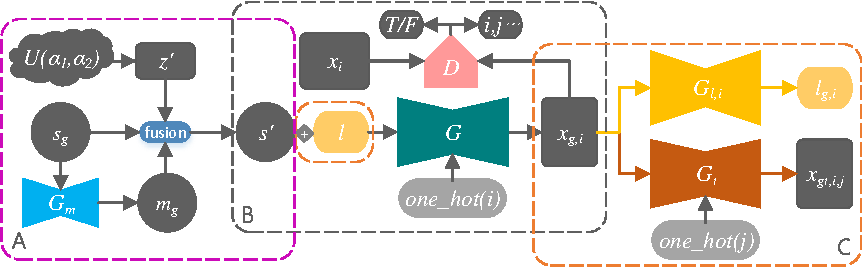
\includegraphics[width=1\columnwidth]{figures/mm_mri_generate_train}
	\caption{Synthesis of multimodal images. Purple box A is the fusion process of structural map and random noise, gray box B is the core process, and yellow box is the optional process. 
		$x_{g,i}$ is the image of modality $i$ generated by generator $G$. 
		$l_{g,i}$ is the lesion label of modality $i$ generated by lesion processor $G_{l,i}$.
		$x_{gt,i,j}$ is the image of modality $j$ translated from modality $i$ by modality translation network $G_t$.
	}
	\label{mm_mri_generate}
\end{figure}
As shown in Fig.~\ref{mm_mri_generate}, we get the structural map $s_g$ through the trained $G_s$ and fuses the random noise, then concatenate the specified lesion label $l$ according to the need. When selecting a lesion tag to guide the synthesis of the lesion, the randomly selected tag may indicate a lesion that is not in the organ described in the structure diagram. We used the mask corresponding to the structure diagram to filter out the labels that the lesion was not within the scope of the organ mask. Then, generator $G$ accepts the onehot condition matrix $one_hot(i)$ after encoding the fusion input, and then decodes to generate the modality $i$ image $x_{g,i}$. The lesion processor $G_{l,i}$ pre-completed training provide the lesions generation guidance loss for $G$ , and the modality translation network $G_t$ pre-completed training provide the registration guidance loss for $G$.

The loss items are as follows, where $d(x_{i})$ and $c(x_{i})$ are the true/false discrimination and category discrimination of the discriminator $D(x_i)$, $d(x_{g, i})$ and $c(x_{g,i})$ are the output of $D(x_{g,i})$. 
\begin{itemize}
	\item{Adversarial loss}
	\begin{equation}
	\begin{split}
	\mathcal{L}_{d2}(D)=\mathbb{E}_{x,s_g,l}[\sum\limits_{i=0}(\Vert{d(x_i)-1}\Vert_{2}^{2}+\Vert{d(x_{g,i})}\Vert_{2}^{2}+\\
	\Vert{c(x_i)-i}\Vert_{2}^{2}+\Vert{c(x_{g,i})-i}\Vert_{2}^{2})],
	\end{split}
	\end{equation}
	\begin{equation}
	\mathcal{L}_{g}(G)=\mathbb{E}_{s_g,l}[\sum\limits_{i=0}(\Vert{d(x_{g,i})-1}\Vert_{2}^{2}+\Vert{c(x_{g,i})-i}\Vert_{2}^{2})].
	\end{equation}
	where $x_{g,i}=G(concat(s',l),one\_hot(i))$,
	$s'=s_g+z'\times(1-m_g)\times(1-s_g)$,
	$m_g=G_m(s_g)$;
%	$[d(x_{i}),c(x_{i})]=D(x_{i})$,$[d(x_{g,i}),c(x_{g,i})]=D(x_{g,i})$;
	$z'\sim\mathcal{U}(\alpha_1,\alpha_2)$ and $\alpha_1=0.5$,$\alpha_2=0.6$;
	$concat()$ is the concatenate function on feturemap channel.
	\item{Lesion generation guidance loss}
	\begin{equation}
	\mathcal{L}_{les}(G)=\mathbb{E}_{s_g,l}[\sum\limits_{i=0}(\Vert{l-l_{g,i}}\Vert_{2}^{2})],
	\end{equation}
	where $l_{g,i}=G_{l,i}(x_{g,i})$.
	\item{Rregistration guidance loss}
	\begin{equation}
	\mathcal{L}_{reg}(G)=\mathbb{E}_{s_g,l}[\sum\limits_{j=0}\sum\limits_{i=0,i\neq j}(\Vert{x_{g,i}-x_{gt,j,i}}\Vert_{2}^{2})],
	\end{equation}
	where $x_{gt,i,j}=G_{t}(x_{g,i},one\_hot(j))$.
\end{itemize}

We can also use the structural feature map extracted from the real image and the real medical image for self-supervised pre-training to accelerate the process of antagonistic training. The loss of the pre-training process is as follows:
\begin{equation}
\mathcal{L}_{p}(G)=\mathbb{E}_{s,l}[\sum\limits_{i=0}(\Vert{x_{g,i}-x_i}\Vert_{2}^{2}+\Vert{x_{g,i}\times m_i-x_{i}\times m_i}\Vert_{2}^{2})].
\end{equation}
where $x_{g,i}=G(concat(s_i',l_i),one\_hot(i))$,$s_i'=s_i+z'\times(1-m_i)\times(1-s_i)$.
。

In the training of SkrGAN\cite{96zhang2019skrgan:}, real sketch training and self-supervision loss are always adopted, which makes the model too few training samples, insufficient training, easy to over-fit and lack of adaptability to the composite sketch, which will eventually lead to the lack of diversity of the composite image. We used real structure diagrams for self-supervised pre-training and a large number of composite structure diagrams for adversarial training, which can not only accelerate the training process, but also enhance the generalization ability of the model.

Fig.~\ref{generated_mri} shows examples of images obtained from all stages on BRATS2015.
\begin{figure}
	\centering
	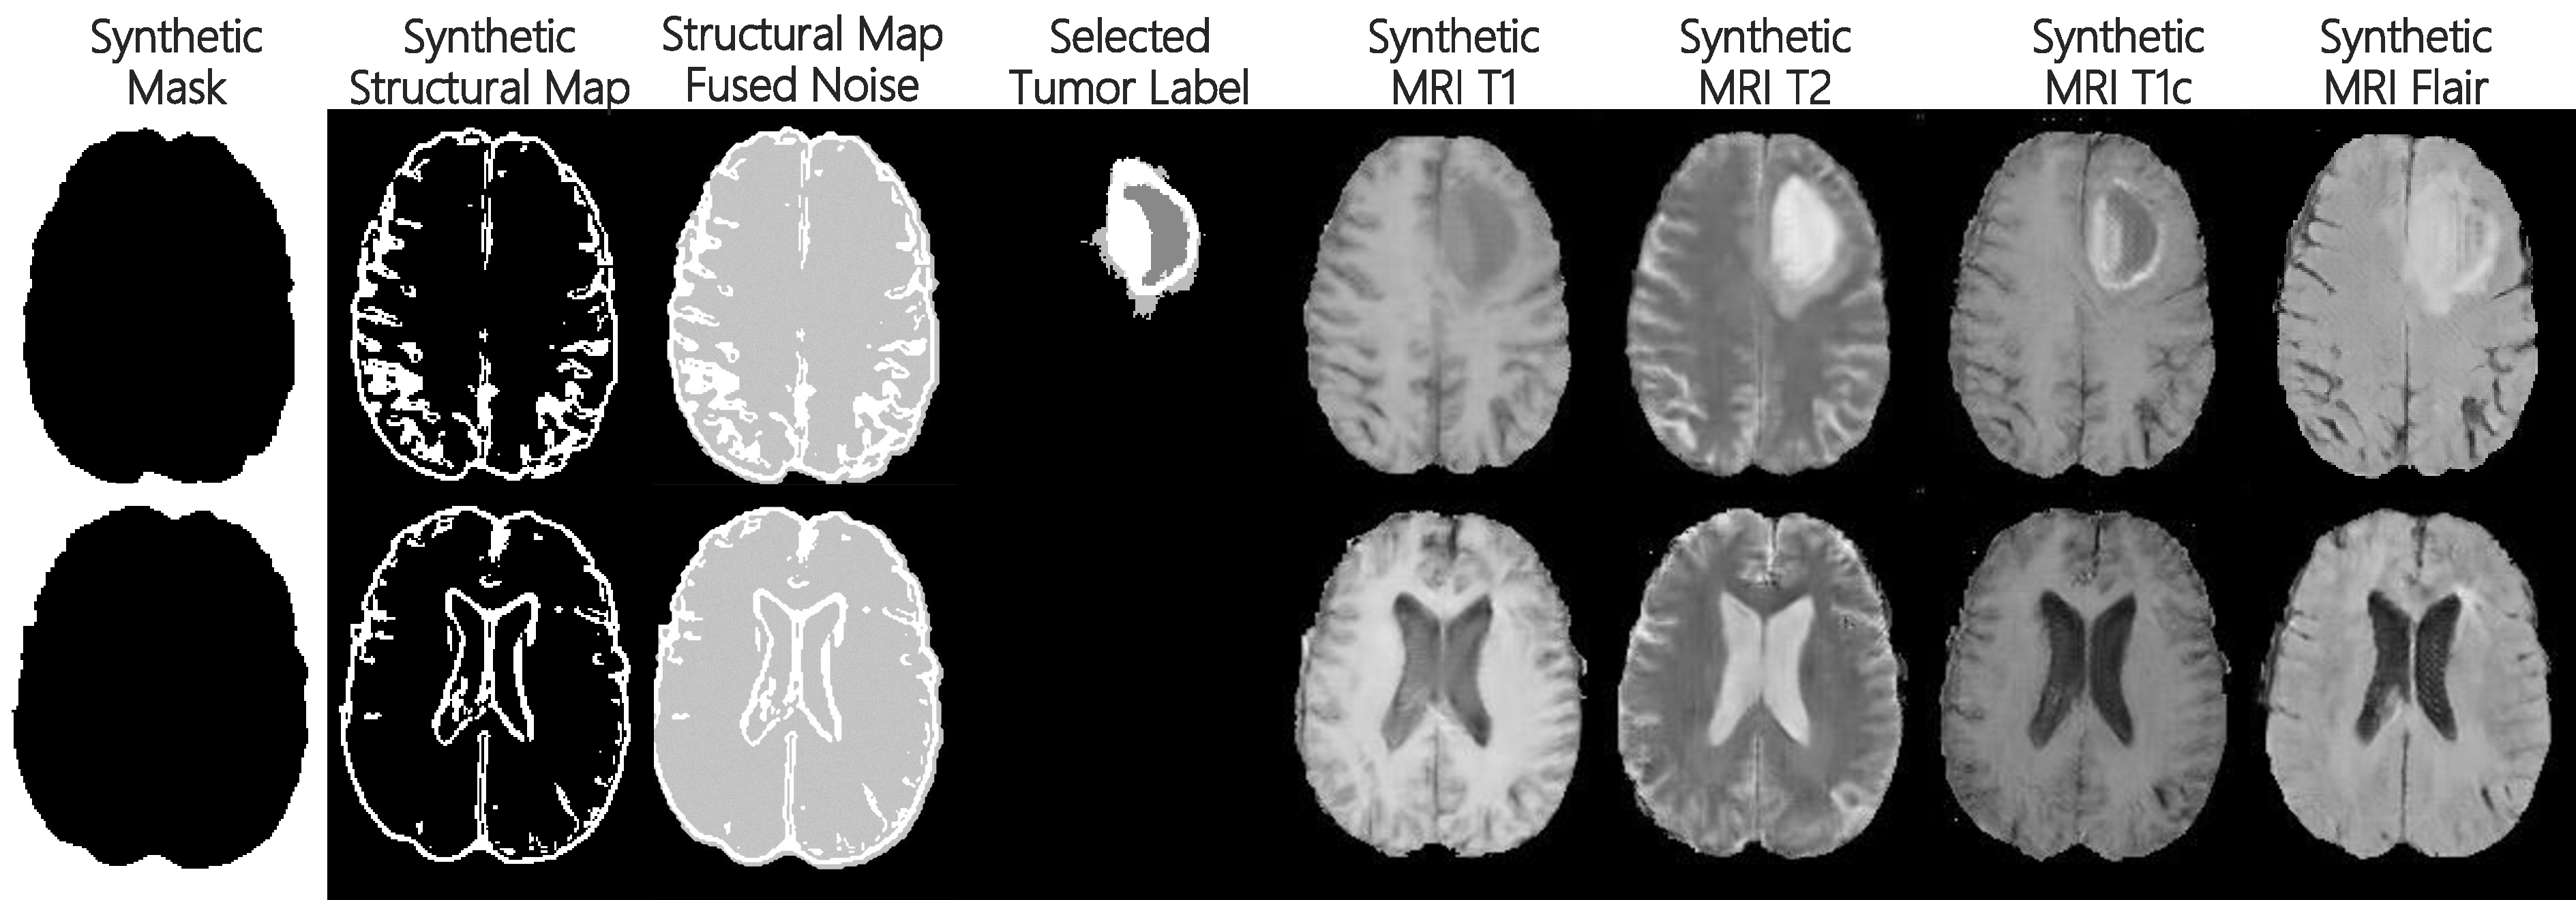
\includegraphics[width=0.7\linewidth]{figures/F_to_MRI}
	\caption{Multimodal images synthesis on BRATS2015.}
	\label{generated_mri}
\end{figure}
\subsection{Translation and lesion processing training}
%As shown in Fig.~\ref{trans_and_segmentation_train},
Before multimodal images synthesis, we perform lesion processing and translation training on real data. 
The translation based on CycleGAN\cite{6zhu2017unpaired} architecture. The losses are as follows:
\begin{itemize}
	\item{Cycle translation adversarial loss}
	\begin{equation}
	\begin{split}
	\mathcal{L}_{cycle}(D_t)=\mathbb{E}_{x,s,l}[\sum\limits_{i=0}(\Vert{d(x_i)-1}\Vert_{2}^{2}+\Vert{d(x_{t,i,j})}\Vert_{2}^{2}+\\
	\Vert{c(x_i)-i}\Vert_{2}^{2}+\Vert{c(x_{t,i,j})-i}\Vert_{2}^{2})],
	\end{split}
	\end{equation}
	\begin{equation}
	\begin{split}
	\mathcal{L}_{cycle}(G_t)=\mathbb{E}_{x}[\sum\limits_{j=0}\sum\limits_{i=0,i\neq j}(\Vert{x_{i}-x_{cr,j,i}}\Vert_{2}^{2})]+\\\mathbb{E}_{s,l}[\sum\limits_{i=0}(\Vert{d(x_{t,i,j})-1}\Vert_{2}^{2}+\Vert{c(x_{t,i,j})-i}\Vert_{2}^{2})],
	\end{split}
	\end{equation}
	where $x_{cr,j,i}=G_t(x_{t,i,j},one\_hot(i)),x_{t,i,j}=G_t(x_{i},one\_hot(j))$,
	$[d(x_{i}),c(x_{i})]=D_t(x_{i})$,$[d(x_{t,i,j}),c(x_{t,i,j})]=D_t(x_{t,i,j})$。
	
	\item{Lesion processing loss}
	\begin{equation}
	\label{lesion segmentation loss}
	\mathcal{L}_{seg}(G_{l,i})=\mathbb{E}_{l,x}[\Vert{l_i-l_{r,i}}\Vert_{2}^{2}],
	\end{equation}
	where $l_{r,i}=G_{l,i}(x_{i})$.
\end{itemize}

\section{EXPERIMENTS}

\subsection{Datasets}
\begin{itemize}
\item \textbf{BRATS2015\cite{91menze:hal-00935640}} includes four registered modalities of T1,T2,T1c,Flair. The training dataset contains 274 3D MRIs per modality, with the size of 155$\times$240$\times$240, and 274 tumor segmentation labels of the same size. We divide the sample into a training set and a test set by 9:1 and construct a 2D dataset from 50 slices of each 55-105 of the 3D MRI. For data preprocessing, we normalize each image.
\item\textbf{Kaggle Chest X-Ray\footnote{https://www.kaggle.com/paultimothymooney/chest-xray-pneumonia }} includes 5863 positive 2D X-ray grayscale images of viral pneumonia, bacterial pneumonia and normal lungs, ranging in size from 384$\times$127 to 2772$\times$2304. During data preprocessing, each image is normalized and scaled to 512$\times$512。
\item\textbf{Kaggle Lung CT\footnote{https://www.kaggle.com/kmader/finding-lungs-in-ct-data/data/}} includes 267 2D CT grayscale images of transverse sections from chest to abdomen, with a size of 512$\times$512. During data preprocessing, each image is normalized.
\item\textbf{DRIVE\footnote{http://www.isi.uu.nl/Research/Databases/DRIVE/}} includes 20 2D   565 $\times $584 color fundus retinal photos in both training set and test set. The training set also inchudes 20 corresponding retinal vascular annotations. In the data preprocessing, each image is standardized, and the unified size interpolation is 512$\times$512.
\item\textbf{FIRE\footnote{https://projects.ics.forth.gr/cvrl/fire/}} includes 268  2D   2912$\times$2912 color fundus retinal photos。 In the data preprocessing, each image is standardized, and the unified size interpolation is 512$\times$512.
\item\textbf{TC Lung CT\footnote{https://tianchi.aliyun.com/competition/entrance/231724/information}} includes 1837 pulmonary 3D CT scans, 1470 in the training set and 145 in the test set. The label information provided in the training set was: center coordinates + diameter (in mm) + category (1-nodule, 2-densification shadow, 3-emphysema or bullae, 5-cord, 31-arteriosclerosis or calcification, 32-lymph node calcification, 33-pleural thickening). We only considered the formation and detection of pulmonary nodules. The 3-channel graph composed of three adjacent slices was input, and the coordinate information of lung nodules of the original intermediate slice was used as the new label. Each image is standardized and scaled to 512$\times$512.
\end{itemize}

\subsection{Experiments settings}
Each experiment was fully trained with more than 100 epochs. The learning rate is 1e-5 without weight decay. We use the Adam optimizer with beta1 of 0.5.Batch size is 4.
We base our results on the current best quality synthesis achieved in SkrGAN\cite{96zhang2019skrgan:}. We used multi-scale structural similarity (MS-SSIM) and FreshetInception distance (FID)\cite{148karras2017progressive} to assess the performance of synthetic medical images. Dice Score\cite {95dice1945measures} and mean square error (MSE) were used to evaluate the segmentation results. Sensitivity, Accuracy and area under the ROC curve (AUC) were used to evaluate vascular annotation results. Accuracy was used to evaluate the classification results of this study. The Average Precision (AP) was used to evaluate the detection results.The evaluation results in this paper are the average of all the modal results on 2D images, and the results of each experiment are the best results reserved after at least 4 training sessions.

\subsection{Ablation experiments on BRATS2015}
\begin{table}[thbp!]
	\newcommand{\tabincell}[2]{\begin{tabular}{@{}#1@{}}#2\end{tabular}}
	\caption{Ablation Experiment on BRATS2015}
	\label{Ablation Experiment Setting on BRATS2015}
	\centering
	\resizebox{\textwidth}{15mm}{
		\begin{tabular}{c|c|c|c|c|c|l}
			%\toprule
			\hline
			Test		&\tabincell{c}{Input \\structural map} &\tabincell{c}{Fusion\\ noise} &\tabincell{c}{with $\mathcal{L}_{reg}$}   &\tabincell{c}{Input lesion \\label and with $\mathcal{L}_{les}$} &\tabincell{c}{Using mask select\\ lesion label} &MS-SSIM   \\
			%\midrule
			\hline
			\tabincell{l}{A}	&$\times$	&$\times$	&$\times$	&$\times$	&$\times$ &0.504 \\
			\tabincell{l}{B}	&$\surd$	&$\times$	&$\times$	&$\times$    &$\times$ &0.654\\
			\tabincell{l}{C}	&$\surd$	&$\surd$	&$\times$	&$\times$	&$\times$ &0.671\\
			\tabincell{l}{D}	&$\surd$	&$\surd$	&$\surd$	&$\times$	&$\times$ &0.674\\
			\tabincell{l}{E}	&$\surd$	&$\surd$	&$\surd$	&$\surd$	&$\times$ &0.673\\
			\tabincell{l}{F}	&$\surd$	&$\surd$	&$\surd$	&$\surd$	&$\surd$ &0.686\\
			\hline
			%\bottomrule
		\end{tabular}
	}
\end{table}
Table~\ref{Ablation Experiment Setting on BRATS2015} shows the setting and results of the ablation experiments of our method.
Fig~\ref{ablation} shows examples of synthetic images generated in ablation experiments. 
Model A replaces the structural feature map with random noise and therefore has no self-supervised pre-training process. Since there is no constraint of the structural feature map on the brain contour, the generated image conforms to the features of MRI, but not to the structural features of the brain. Model B used structural features to represent the input but did not fuse random noise. After the training of epoch, which was the same as other experiments, poor quality was synthesized and the registration effect of the generated images was not very good, and no obvious lesion information was synthesized. Model C has no modal registration loss, and the resulting image registration effect is not very good, especially the edge details. In model D, there was no loss of guidance for lesion generation. It can be seen that the lesions in the generated images were random and exaggerated, which did not match the input lesion label. Model E had no mask to filter the input labels, and it was easy to see that the synthetic tumor was beyond the contours of the brain. Model F adopts the complete scheme of this study to synthesize the lesion information consistent with the input lesion label, with high registration degree and high synthesis quality. It can be seen from the visual comparison that all the improvements in this study have improved the authenticity of the synthesized image. However, if the lesion label is added and the lesion generation guidance is used to guide the loss, if the lesion label is not screened by mask, the image with similar unreasonable structure as shown in model E may be generated.
\begin{figure}
	\centering
	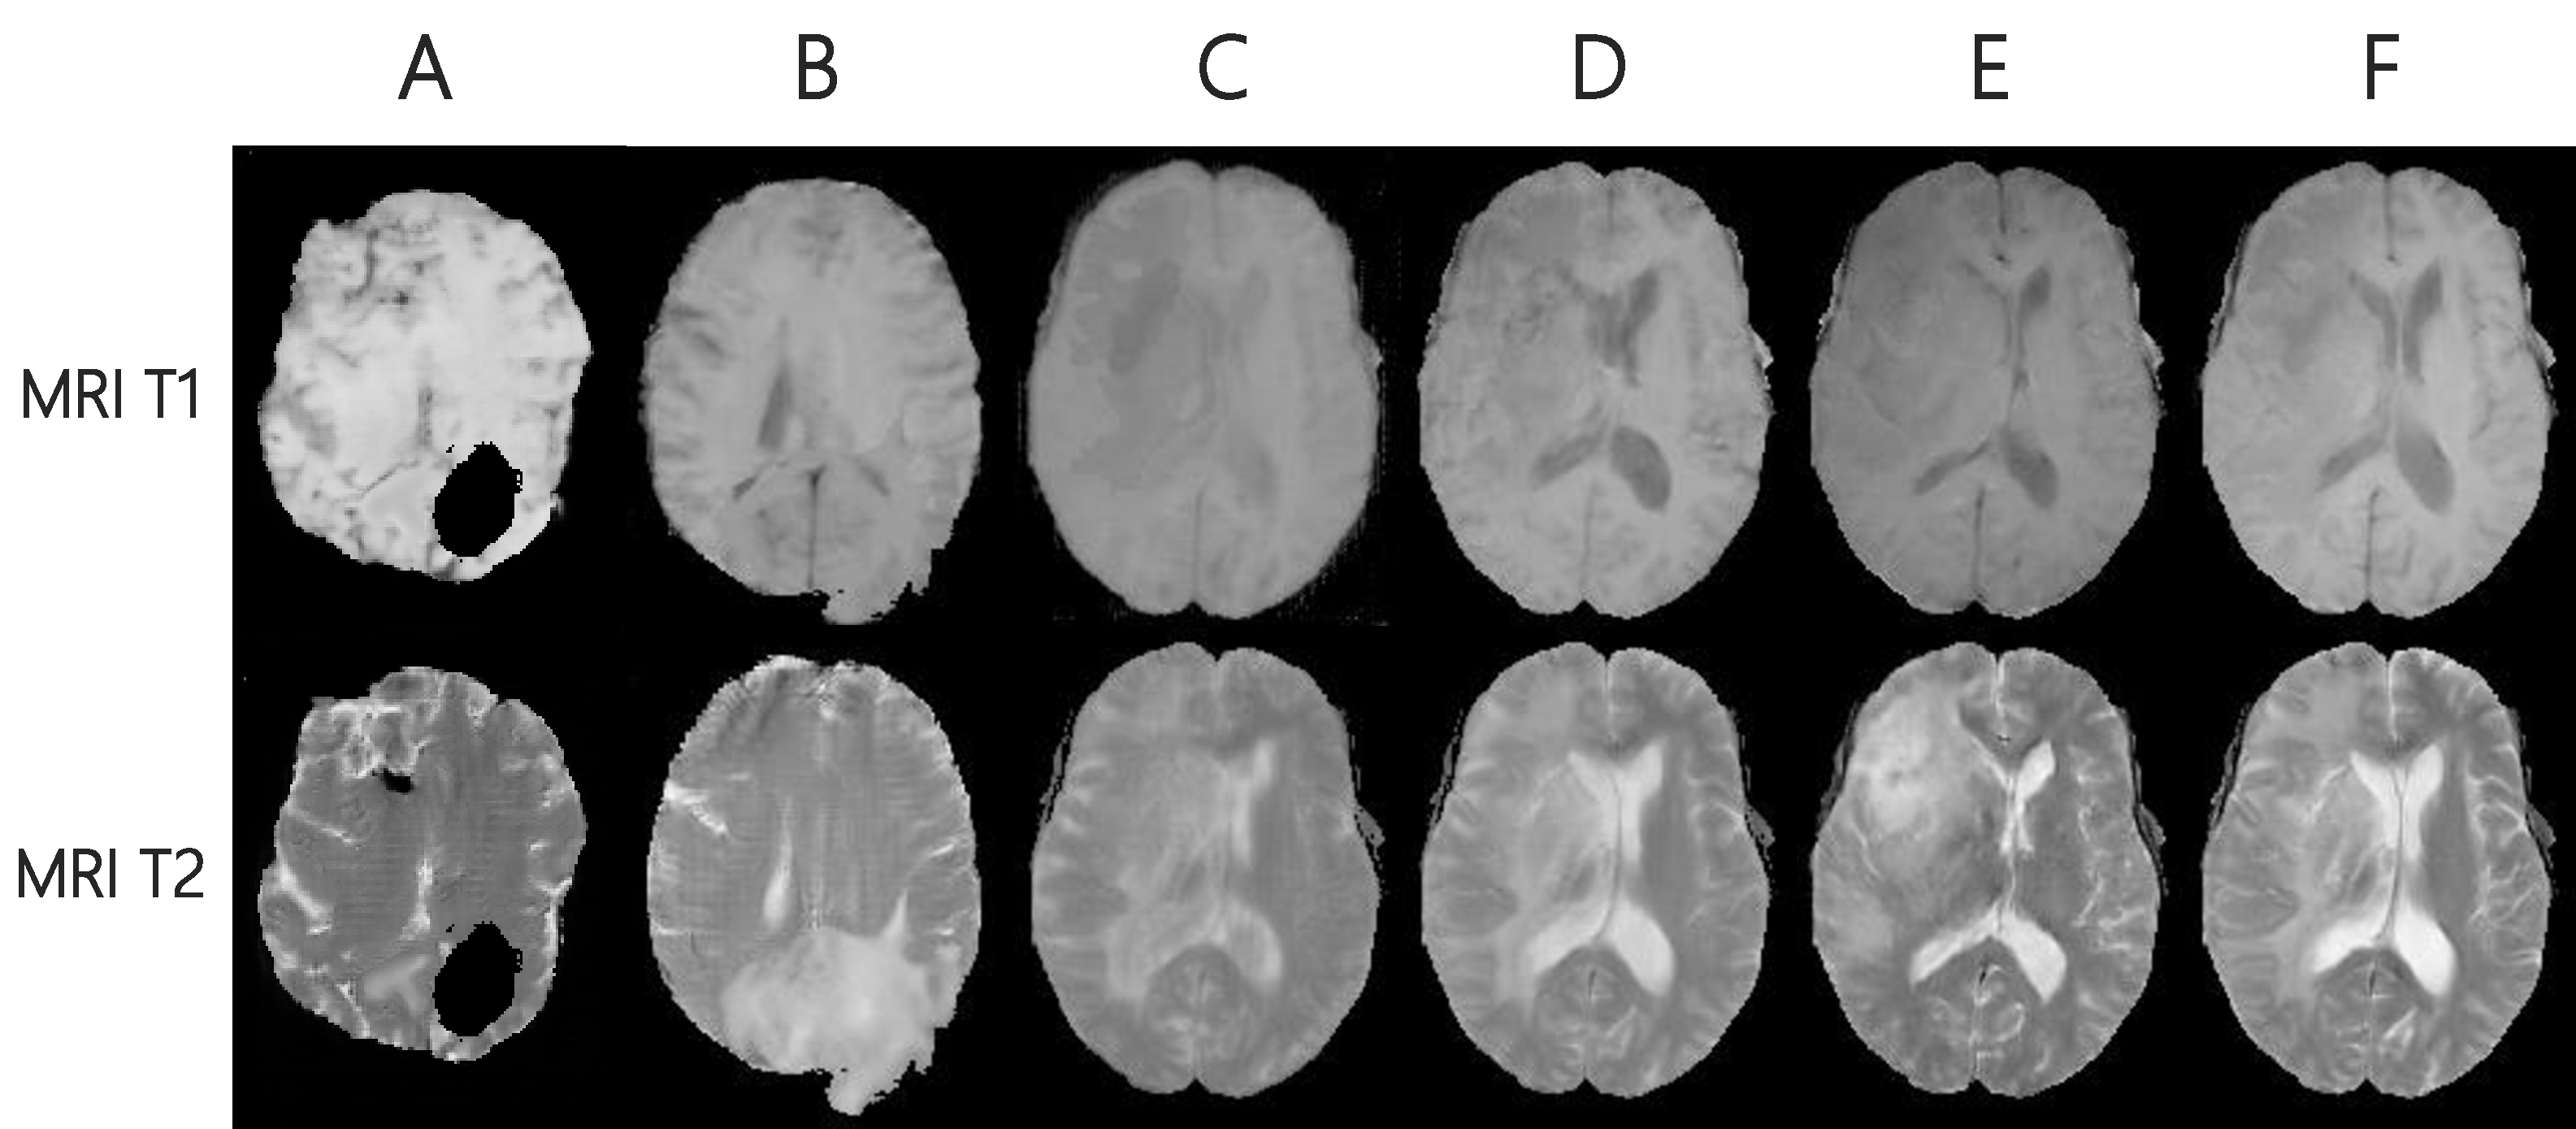
\includegraphics[width=0.67\linewidth]{figures/ablation}
	\caption{Synthetic images of ablation experiments.}
	\label{ablation}
\end{figure}

\subsection{Evaluation of lesion effectiveness on BRATS2015}
\label{label gen methods tests}

\begin{table}
	\begin{center}
		\caption{Lesion generation methods experiments.}
		\label{label_test}
		\begin{tabular}{lccc}
			\hline
			\rule{0pt}{12pt}
			Testing Dataset &MSE   &Dice score
			\\
			\hline
			\\[-6pt]
			real 		   				&0.027 &0.915 \\							
			synthetic     			&\textbf{0.043} &\textbf{0.838} \\
			\hline
			\\[-6pt]
		\end{tabular}
	\end{center}
\end{table}
\begin{figure}[thbp!]
	\centering
	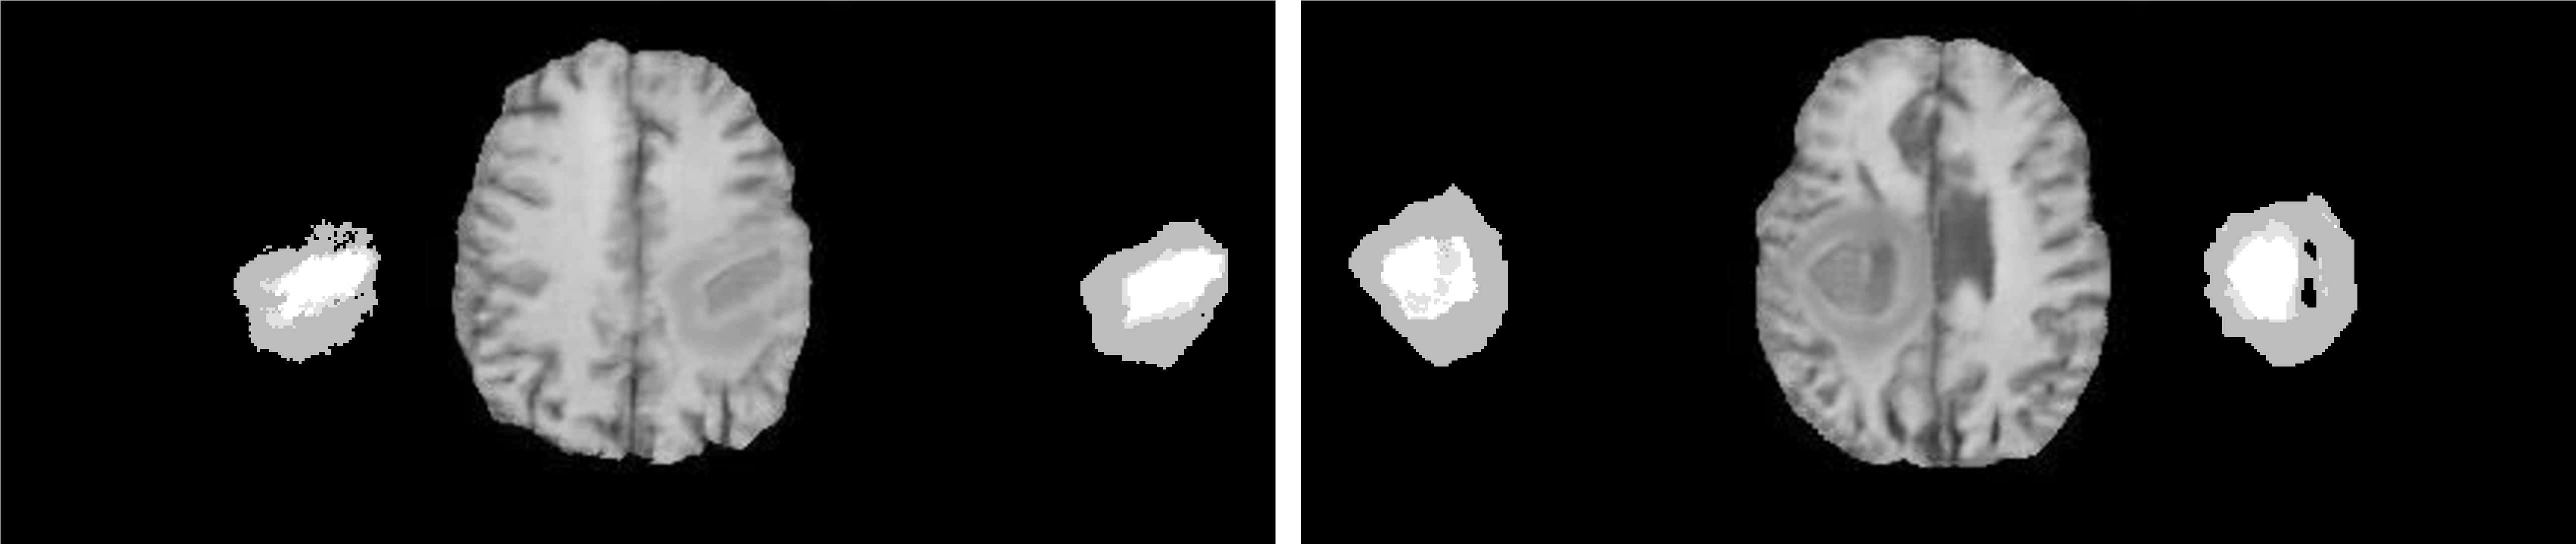
\includegraphics[width=0.65\linewidth]{figures/seg_res}
	\caption{The segmentation results of synthetic MRI with brain tumor segmentor. Follows are the input tumor segmentation label, the synthesized MRI T1, the segmentation result.}
	\label{seg_res}
\end{figure}

As reported in Table~\ref{label_test}, the segmentation test results of the segmentor trained on real data reach an MSE of 0.026 and Dice score of 0.915. From the segmentation results, the splitter trained with real data can be used on the synthesized data, which indicates that the synthesized data and the real data have a very high degree of similarity, and the synthesized lesions and the real lesions are similar enough for the splitter to recognize the synthetic lesions and non-focal parts. This suggests that synthetic lesions are effective.

\subsection{Evaluation of synthetic images quality }
\begin{table}[thbp!]
	\newcommand{\tabincell}[2]{\begin{tabular}{@{}#1@{}}#2\end{tabular}}
	\begin{center}
		\caption{Evaluation of synthetic images quality (A)}
		\label{evalu_on_all_dataset1}
		\resizebox{\textwidth}{12mm}{
			\begin{tabular}{ll|llllll}
				\hline
				\rule{0pt}{10pt}
				Dataset &Metric &Ours &SkrGAN\cite{96zhang2019skrgan:} &DCGAN\cite{97radford2015unsupervised} &ACGAN\cite{98odena2016conditional} &WGAN\cite{99arjovsky2017wasserstein} &PGGAN\cite{100karras2017progressive}\\
				\hline
				\multirow{2}*{\tabincell{l}{\textbf{Kaggle Chest}\\\textbf{X-ray}}}
				&MS-SSIM ↑ &0.597 &0.506 &0.269 &0.301 &0.401 &0.493 \\
				&FID ↓ &102.5 &114.6 &260.3 &235.2 &300.7 &124.2\\
				\hline
				\multirow{2}*{\tabincell{l}{\textbf{Kaggle Lung}\\\textbf{CT}}}
				&MS-SSIM ↑ &0.473 &0.359 &0.199 &0.235 &0.277 &0.328 \\
				&FID ↓ &66.91 &79.97 &285.0 &222.5 &349.1 &91.89\\
				\hline
				\\[-6pt]
			\end{tabular}
		}
	\end{center}
\end{table}

\begin{table}[thbp!]
	\newcommand{\tabincell}[2]{\begin{tabular}{@{}#1@{}}#2\end{tabular}}
	\begin{center}
		\caption{Evaluation of synthetic images quality (B)}
		\label{evalu_on_all_dataset2}
		\resizebox{0.7\textwidth}{17mm}{
			\begin{tabular}{ll|llll}
				\hline
				\rule{0pt}{10pt}
				Dataset &Metric &Ours$^+$ &Ours &SkrGAN$^*$ &GAN$^\#$\\
				\hline
				\multirow{2}*{\tabincell{l}{\textbf{DRIVE+FIRE}\\\textbf{Color Fundus}}}
				&MS-SSIM ↑  &-     &0.607 &0.584 &0.392\\
				&FID ↓      &-     &30.13 &37.91 &227.41\\
				\hline
				\multirow{2}*{\tabincell{l}{\textbf{BRATS2015 }\textbf{MRI}}}
				&MS-SSIM ↑  &0.692 &0.686 &0.653 &0.504\\
				&FID ↓      &20.15 &21.87 &28.76 &124.53\\
				\hline
				\multirow{2}*{\tabincell{l}{\textbf{TC Lung }\textbf{CT}}}
				&MS-SSIM ↑  &-     &0.676 &0.667 &0.543\\
				&FID ↓      &-     &27.40 &29.81 &113.65\\
				\hline
				\\[-6pt]
			\end{tabular}
		}
		\footnotesize
		\item[+]  the evaluation of the synthetic tumor, that is, the evaluation of the tumor excised from the synthetic data set image and the original data set image based on the lesion label.
		\item[\#] The result of basic GAN using adversarial loss.
		\item[*] The result of reproduce SkrGAN using the input of the inverse binary image of our structure map (0 and 1 pixel value inversion).
	\end{center}
\end{table}
As shown in Table~\ref{evalu_on_all_dataset1},~\ref{evalu_on_all_dataset2}, our method was quantitatively evaluated on each dataset and compared with the most advanced current methods. Combined with the results in tables and the visual comparison in Fig.~\ref{evalu_compare}, the quality of the composite image input with structural feature diagram is much better than that of the composite image input with random noise. The generalization ability of the model is stronger when the structure feature map is processed by fusion noise than when it is not processed or treated by binary inversion. Self - supervised pre - training can improve the quality of composite image obviously on small data sets. Compared with the sketch of SkrGAN and other random noise input, the structural feature map, self-supervised pre-training, lesion loss and other measures adopted by us make the synthetic medical image in this study of higher quality and closer to the real image
\begin{figure}
	\centering
	\includegraphics[width=0.95\linewidth]{figures/evalu_compare}
	\caption{Visual contrast of Synthetic images.(a) Synthetic image of PGGAN\cite{100karras2017progressive}.(b) Synthetic image of WGAN \cite{99arjovsky2017wasserstein}.(c) Synthetic image of DCGAN\cite{97radford2015unsupervised}.(d) Synthetic image of ACGAN\cite{98odena2016conditional}.(e) Synthetic image of SkrGAN\cite{96zhang2019skrgan:}, the input sketch and the sketch binary inversion image.(f) Our synthetic image, the input structural map fusioned the noise and the original structural map.}
	\label{evalu_compare}
\end{figure}

\subsection{Evaluation of synthetic data availability}
\begin{table}
	\begin{center}
		{\caption{Synthetic data availability verification on BRATS2015.}\label{availability_test}}
		\begin{tabular}{lllllcc}
			\hline
			\rule{0pt}{12pt}
			NO. &Real &Synthetic & Enhanced & Mix  & MSE &Dice score\\
			\hline
			\\[-6pt]
			\quad 1 & $\times$1  	 	& 0 		&0 			&- &0.027 &0.915 \\
%			\quad2 & $\times$50\% 	 & 0  		&0 			&- &0.032 &0.902 \\
			\quad3 &0 	 	 & $\times$1  	&0 			&- &0.205 &0.708 \\
%			\quad4 &0 	 	 & $\times$2  	&0 			&$\mathcal{M}$ &0.206 &0.736 \\
%			\quad5 &0 		 & $\times$3  	&0 			&$\mathcal{M}$ &0.205 &0.754 \\
%			\quad6 & $\times$10\% 	 & $\times$1  	&0 			&$\mathcal{S}$ &0.031 &0.908 \\
%			\quad7 & $\times$10\% 	 & $\times$2   &0 			&$\mathcal{S}$ &0.028 &0.907 \\
%			\quad8 & $\times$10\% 	 & $\times$3   &0 			&$\mathcal{S}$ &0.030 &0.907 \\	
			\quad9 & $\times$20\% 	 & $\times$80\% 	&0  		&$\mathcal{M}$ &0.041 &0.850 \\
			\quad10& $\times$50\% 	 & $\times$50\% 	&0  		&$\mathcal{M}$ &0.031 &0.904 \\
			\quad11& $\times$80\% 	 & $\times$20\% 	&0  		&$\mathcal{M}$ &0.028 &0.913 \\
			\quad12& $\times$1 	 	& $\times$20\% &0  		&$\mathcal{M}$ &0.025 &0.921 \\
			\quad13& $\times$1 	 	& $\times$50\% &0  		&$\mathcal{M}$ &\textbf{0.021} &\textbf{0.939} \\
%			\quad14& $\times$1 	 	& $\times$80\% &0  		&$\mathcal{M}$ &0.026 &0.916 \\
			\quad15& $\times$1 	 	& $\times$1    &0   		&$\mathcal{M}$ &0.022 &0.934 \\
			\quad16& $\times$1 	 	& $\times$2   &0 			&$\mathcal{M}$ &0.023 &0.929 \\
			\quad17& $\times$1 	 	& $\times$3   &0 			&$\mathcal{M}$ &0.024 &0.925 \\	
			\quad18& $\times$1 	 	&0 		&  $\times$20\%	 	&$\mathcal{M}$ &0.027 &0.916 \\
			\quad19& $\times$1 	 	&0 		&  $\times$50\% 	&$\mathcal{M}$ &0.025 &0.920 \\
%			\quad20& $\times$1    	&0 		&  $\times$80\% 	&$\mathcal{M}$ &0.026 &0.920 \\
			\quad21& $\times$1 	 	&0 		&  $\times$1    &$\mathcal{M}$ &0.025 &0.919 \\
			\quad22& $\times$1 	 	&0 		&  $\times$2   &$\mathcal{M}$ &0.026 &0.919 \\
			\quad23& $\times$1 	 	&0 		&  $\times$3   &$\mathcal{M}$ &0.026 &0.918 \\			
			\quad24& $\times$1 	 	& $\times$1 	&0  		&$\mathcal{R}$ &0.195 &0.795 \\
			\quad25& $\times$1 	 	& $\times$1 	&0  		&$\mathcal{S}$ &\textbf{0.021} &\textbf{0.940}
			\\
			\hline
			\\[-6pt]
			\multicolumn{7}{l}{$\mathcal{M}:$ random mixing\ \
				$\mathcal{S}:$ synthetic first\ \
				$\mathcal{R}:$ real first}
		\end{tabular}
	\end{center}
\end{table}
\begin{table}[thbp!]
	\newcommand{\tabincell}[2]{\begin{tabular}{@{}#1@{}}#2\end{tabular}}
	\begin{center}
		\caption{Synthetic data availability verification on DRIVE.}
		\label{DRIVE_availability_test}
		\begin{tabular}{clccc}
			\hline
			\rule{0pt}{12pt}
			Train Data  &Test Data &Sensitivity &Accuracy &AUC\\
			\hline
			\tabincell{c}{DRIVE Training Set}  	 	&  DRIVE Test Set 	&0.7781 &0.9477 &0.9705
			\\
			\tabincell{c}{DRIVE Training Set+2000\\SkrGAN Synthetic Images}	 &  DRIVE Test Set 	& 0.8464 &0.9513 &0.9762 \\
			\tabincell{c}{DRIVE Training Set+2000\\SkrGAN$^*$ Synthetic Images}	 &  DRIVE Test Set 	& 0.8297 &0.9428 &0.9732 \\
			\tabincell{c}{DRIVE Training Set+2000\\Our Synthetic Images}	&  DRIVE Test Set 	& 0.8416 &0.9518 &0.9749 \\	
			\hline
		\end{tabular}
		\footnotesize
		\item[*] The result of reproduce SkrGAN using the input of the inverse binary image of our structure map (0 and 1 pixel value inversion).
	\end{center}
\end{table}
\begin{table}[thbp!]
	\newcommand{\tabincell}[2]{\begin{tabular}{@{}#1@{}}#2\end{tabular}}
	\begin{center}
		\caption{Synthetic data availability verification on Kaggle Chest X-Ray.}
		\label{X-Ray_availability_test}
		\begin{tabular}{clllc}
			\hline
			\rule{0pt}{12pt}
			Train Data  &Test Data &Accuracy \\
			\hline
			\tabincell{c}{Kaggle Chest X-Ray\\ Training Set}  	 	&\tabincell{c}{ Kaggle Chest X-Ray\\Test Set }	&0.804 
			\\
			\tabincell{c}{Kaggle Chest X-Ray Training Set\\+ 2000 Synthetic Images}	& \tabincell{c}{Kaggle Chest X-Ray\\Test Set } 	& 0.818 \\	
			\hline
		\end{tabular}
	\end{center}
\end{table}
\begin{table}[thbp!]
	\newcommand{\tabincell}[2]{\begin{tabular}{@{}#1@{}}#2\end{tabular}}
	\begin{center}
		\caption{Synthetic data availability verification on TC Lung CT.}
		\label{TC_availability_test}
		\begin{tabular}{clllc}
			\hline
			\rule{0pt}{12pt}
			Train Data  &Test Data & AP \\
			\hline
			\tabincell{c}{TC Lung CT \\Training Set}  	 	&\tabincell{c}{TC Lung CT \\Test Set} 	&0.574 
			\\
			\tabincell{c}{TC Lung CT Training Set\\+ 20000 Synthetic Images}	&\tabincell{c}{TC Lung CT \\Test Set}  	& 0.592 \\	
			\hline
		\end{tabular}
	\end{center}
\end{table}
As shown in Table~\ref{availability_test}, we mix real BRATS2015 training data with BRATS synthetic data in different amounts, then use the mixed dataset for segmentation training using the multiple segmentors method, and finally evaluate the segmentation ability of the model on the real BRATS2015 test dataset. All experiments are fully trained with the same number of iterations, which is equal to the number of 100 epochs on the BRATS2015 training dataset. At the same time, we set up three data mixing modes: random mixing, real data training first, and synthetic data training first. In the real-first experiments and synthetic-first experiments, the training iteration number of data from different sources is proportional to the quantity of data. Except for the conditions listed in the table, the other conditions are identical.

As reported in Table~\ref{availability_test}, if there is a large quantity of real data, a small quantity of synthetic data can be used as enhanced data, or a large quantity of synthetic data can be used for pre-training and then training on real data. If there are fewer real data, a large number of synthetic data can be used for pre-training, and then, fine-tuning can be performed on a small quantity of real data, whose results can compete with the results on complete real data; this conclusion is consistent with \cite{4shin2018medical}. We do not recommend using synthetic data completely for training and also do not recommend using synthetic data for supplementary training.

As shown in Table~\ref{DRIVE_availability_test},\ref{X-Ray_availability_test},\ref{TC_availability_test}, we performed other medical image processing tasks with the medical images synthesized on other data sets. The results in the table show that our synthesized data can improve the generalization ability of the model in these tasks, which indicates that our synthesized data are available and the synthesized lesions are effective.

\section{CONCLUSION}
In short, we propose a structural map extraction method to extract anatomical structure information directly from medical images without training or additional label data.
We propose a structure feature map generation method to generate structural maps from multidimensional normal distribution matrixes.
We realize the synthesis of registered multimodal images from a random normal distribution matrix through unsupervised training, which can add the lesion information freely.
We verify that synthetic images can be used as pre-training data or enhanced data for intelligent medical image processing tasks and can significantly improve the generalization ability of the model through lesion segmentation experiments.

%
% ---- Bibliography ----
%
% BibTeX users should specify bibliography style 'splncs04'.
% References will then be sorted and formatted in the correct style.
%
\bibliographystyle{splncs04}
\bibliography{mybibliography}


\end{document}
